\documentclass[conference]{IEEEtran}
\IEEEoverridecommandlockouts
\usepackage[utf8]{inputenc}
\usepackage[spanish,es-tabla]{babel}
\usepackage{amsmath,amssymb,amsfonts}
\usepackage{algorithmic}
\usepackage{graphicx}
\usepackage{textcomp}
\usepackage{xcolor}
\usepackage{booktabs}
\usepackage{microtype}
\usepackage{url}
\usepackage{listings}

\lstset{
    basicstyle=\ttfamily\footnotesize,
    breaklines=true,
    frame=single,
    backgroundcolor=\color{gray!10},
    keywordstyle=\color{blue},
    commentstyle=\color{gray},
    stringstyle=\color{teal}
}

\def\BibTeX{{\rm B\kern-.05em{\sc i\kern-.025em b}\kern-.08em
    T\kern-.1667em\lower.7ex\hbox{E}\kern-.125emX}}

\begin{document}

\title{Despliegue y Validación en Entorno Local de una Arquitectura de Microservicios para Comercio Electrónico con Mediador Centralizado y Persistencia Aislada}

\author{
\IEEEauthorblockN{Mark Osorio}
\IEEEauthorblockA{\textit{Facultad de Ingeniería} \\
\textit{Universidad Mesoamericana (UMES)}\\
Quetzaltenango, Guatemala \\
osoriomark@umes.edu.gt}
\and
\IEEEauthorblockN{Cátedra: Arquitectura de Sistemas I}
\IEEEauthorblockA{\textit{Ingeniería en Sistemas, Informática y Ciencias de la Computación} \\
\textit{Universidad Mesoamericana}\\
Ciclo 2026 -- Proyecto Final}
}

\maketitle

\begin{abstract}
Este informe de avance técnico documenta el diseño, la puesta en marcha local y la verificación funcional de un ecosistema distribuido de comercio electrónico orientado a microservicios. La arquitectura implementada se compone de tres proyectos de backend independientes: un servicio mediador (Broker) que funge como punto único de entrada y gestor de autenticación basado en tokens JWT, un microservicio de Productos desarrollado bajo el patrón Modelo-Vista-Controlador (MVC), y un microservicio de Pedidos estructurado en arquitectura por capas. La persistencia se diseñó mediante bases de datos aisladas en MySQL 8.4 gestionadas por medio de TypeORM. La orquestación completa del entorno se resolvió mediante Docker Compose, garantizando aislamiento de redes y control estricto de exposición de puertos. Las pruebas de integración se validaron con Postman contra la dirección local del broker, verificando tanto el rechazo sistemático de peticiones anónimas como el flujo transaccional de verificación y descuento de existencias.
\end{abstract}

\begin{IEEEkeywords}
Arquitectura de Microservicios, API Gateway, Broker, Autenticación JWT, Docker Compose, Modelo-Vista-Controlador (MVC), Arquitectura por Capas, TypeORM, Postman.
\end{IEEEkeywords}

\section{Introducción}
El diseño de sistemas empresariales modernos exige desacoplar las responsabilidades de negocio para garantizar escalabilidad, tolerancia a fallos e independencia en el ciclo de vida del software. Frente a los modelos monolíticos tradicionales, las arquitecturas orientadas a servicios distribuidos permiten aislar dominios funcionales críticos, como la gestión de catálogos y el procesamiento transaccional de órdenes de compra.

En el marco del proyecto de la cátedra de Arquitectura de Sistemas I de la Universidad Mesoamericana, se estableció como requisito la construcción individual de una plataforma de comercio electrónico compuesta por tres componentes de backend desacoplados, sin interfaz gráfica de usuario, demostrable exclusivamente mediante herramientas de prueba de API (Postman) y orquestada en contenedores. 

El presente informe detalla la fase inicial del proyecto, enfocada en:
\begin{enumerate}
    \item La definición de los límites arquitectónicos de cada servicio.
    \item La configuración de la persistencia aislada con mapeo objeto-relacional (ORM).
    \item La orquestación integral en entorno local con Docker y Docker Compose.
    \item La verificación empírica de las reglas de autenticación e integración interservicios.
\end{enumerate}

\section{Diseño Arquitectónico del Ecosistema}
El sistema se organiza bajo el patrón de diseño de puerta de enlace o mediador (\textit{Broker/Mediator Pattern}), en el cual ningún servicio de negocio se expone directamente a los clientes externos. Toda solicitud proveniente del exterior debe atravesar el broker, que asume la responsabilidad de autenticación previa a cualquier redirección.

\subsection{Microservicio Broker / Mediador (Puerto 3000)}
El Broker actúa como fachada perimetral y punto de entrada único (\textit{Single Point of Entry}) al sistema. Se implementó utilizando NestJS sobre Node.js y TypeScript. Su comportamiento se apega rigurosamente a las siguientes directrices:
\begin{itemize}
    \item \textbf{Cero lógica de negocio:} No procesa reglas comerciales, cálculos de inventario ni transacciones financieras.
    \item \textbf{Autenticación centralizada:} Valida la presencia e integridad de tokens JWT transmitidos en la cabecera HTTP \texttt{Authorization: Bearer <token>} mediante la biblioteca criptográfica \texttt{jose}.
    \item \textbf{Enrutamiento transparente:} Redirige las solicitudes validadas hacia los servicios internos (\texttt{http://productos:3001} y \texttt{http://pedidos:3002}) a través de un proxy HTTP interno, inyectando un token de firma de servicio (\texttt{SERVICIO\_TOKEN}) para autenticar la comunicación interna.
    \item \textbf{Manejo de acceso:} Incorpora un subsistema de credenciales para usuarios administradores y clientes, permitiendo revocar accesos y denegar operaciones a identidades suspendidas.
\end{itemize}

\subsection{Microservicio de Productos (Puerto 3001)}
Encargado exclusivo de la administración del catálogo y el control de existencias. Su diseño sigue el patrón arquitectónico \textbf{Modelo-Vista-Controlador (MVC)}:
\begin{itemize}
    \item \textbf{Modelo:} Entidad \texttt{Producto} mapeada con TypeORM hacia la tabla correspondiente, almacenando identificador autoincremental, nombre, precio unitario y existencias (\textit{stock}).
    \item \textbf{Vista:} Clases de transferencia de datos (DTOs) y transformadores REST (\texttt{ProductoVista}, \texttt{DescuentoVista}) que moldean las respuestas JSON hacia el cliente, asegurando la serialización y ocultamiento de atributos internos.
    \item \textbf{Controlador:} Expone endpoints para el CRUD completo de productos y validaciones numéricas estrictas ($precio > 0$, $stock \ge 0$). Asimismo, implementa la ruta crítica de descuento de existencias requerida por el servicio de pedidos.
\end{itemize}

\subsection{Microservicio de Pedidos (Puerto 3002)}
Responsable del registro y control de ciclo de vida de las compras. Está construido bajo una \textbf{Arquitectura en Capas} que desacopla la recepción HTTP de la lógica de aplicación y el acceso a datos:
\begin{itemize}
    \item \textbf{Capa de Presentación:} Controladores que capturan las peticiones de creación y consulta de pedidos, validando los parámetros de entrada mediante \texttt{class-validator}.
    \item \textbf{Capa de Negocio / Dominio:} Orquesta la lógica del pedido. Antes de asentar la orden, invoca al cliente de productos a través del Broker para verificar la existencia del artículo y la disponibilidad del stock solicitado.
    \item \textbf{Capa de Persistencia / Datos:} Repositorio TypeORM que almacena los registros con identificador UUIDv4, estado de la orden (\texttt{PENDIENTE}, \texttt{CONFIRMADO}, \texttt{RECHAZADO}) y fecha de creación.
    \item \textbf{Idempotencia y Manejo de Fallos:} Si la consulta de inventario o el descuento falla (por existencia insuficiente o tiempo de espera agotado), la orden se transiciona al estado correspondiente sin inconsistencias en el inventario.
\end{itemize}

\subsection{Persistencia y Aislamiento de Datos}
Para cumplir con el principio de persistencia políglota y bases de datos independientes por microservicio, se configuró una instancia de MySQL 8.4 que aloja tres esquemas completamente separados:
\begin{itemize}
    \item \texttt{broker}: Almacena usuarios, credenciales hasheadas y estado de autenticación.
    \item \texttt{productos}: Almacena catálogo, descripciones, precios e inventario físico.
    \item \texttt{pedidos}: Almacena órdenes de compra, referencias cruzadas y estados de procesamiento.
\end{itemize}
Cada base de datos cuenta con un usuario SQL independiente con privilegios acotados únicamente a su esquema, imposibilitando la lectura cruzada de tablas a nivel de base de datos.

\section{Orquestación y Puesta en Marcha con Docker}
La totalidad de los servicios se empaquetó en contenedores Docker y se orquestó mediante un archivo \texttt{compose.yaml}.

\subsection{Aislamiento de Redes y Control de Puertos}
En una arquitectura de microservicios robusta, los servicios de dominio no deben ser alcanzables directamente desde redes públicas. Por ello, la directiva de puertos de Docker Compose se configuró de la siguiente forma:
\begin{itemize}
    \item \textbf{Broker:} Publica el puerto \texttt{127.0.0.1:3000:3000}. Es la única compuerta accesible desde la máquina anfitriona y herramientas externas.
    \item \textbf{Productos:} Escucha en el puerto \texttt{3001} únicamente dentro de la red privada de Docker (\texttt{tienda}). No expone puertos al host.
    \item \textbf{Pedidos:} Escucha en el puerto \texttt{3002} dentro de la red privada de Docker (\texttt{tienda}). No expone puertos al host.
    \item \textbf{MySQL:} Expone el puerto \texttt{3306} para tareas de mantenimiento local, implementando una directiva de \textit{healthcheck} con \texttt{mysqladmin ping} para asegurar que los servicios dependientes arranquen únicamente tras la disponibilidad del motor SQL.
\end{itemize}

\subsection{Evidencias de Ejecución}
La Fig.~\ref{fig:terminal} muestra la salida de la consola durante la recreación y el levantamiento ordenado de los tres microservicios en segundo plano, así como el listado de estado generado con el comando \texttt{docker compose ps}. Se evidencia que los cuatro contenedores (\texttt{tienda-mysql-1}, \texttt{tienda-broker-1}, \texttt{tienda-pedidos-1} y \texttt{tienda-productos-1}) se encuentran en ejecución activa (\textit{healthy} y \textit{Up}).

\begin{figure}[htbp]
\centering
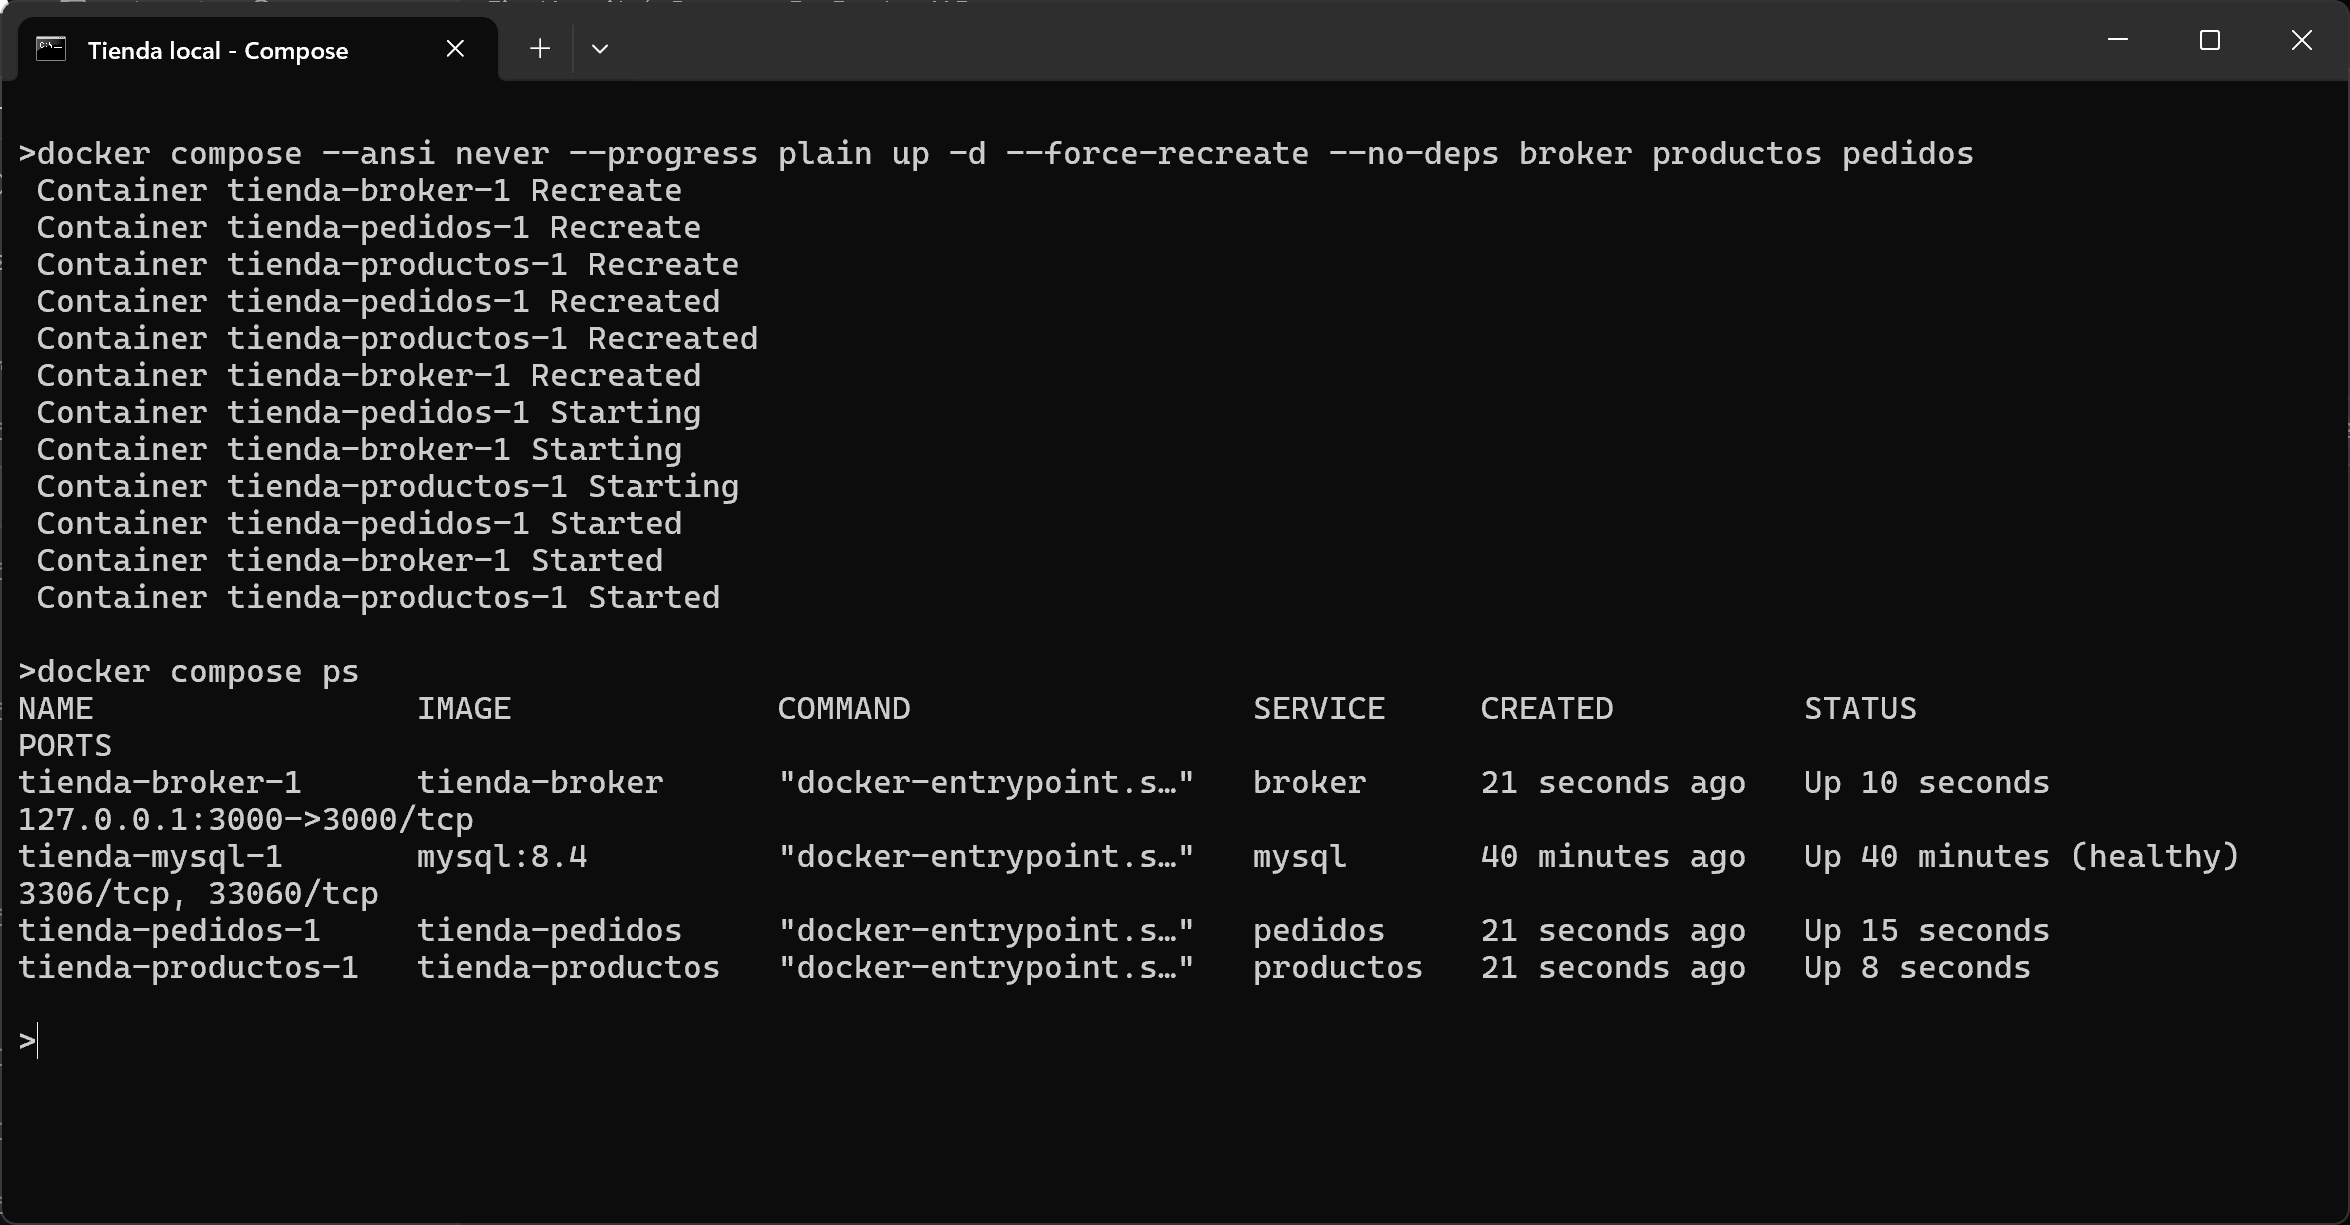
\includegraphics[width=\columnwidth]{fig/ag-terminal-compose.png}
\caption{Consola de comandos evidenciando la recreación de contenedores y la verificación de estados con \texttt{docker compose ps}.}
\label{fig:terminal}
\end{figure}

Por su parte, la Fig.~\ref{fig:docker} presenta el panel gráfico de Docker Desktop dentro de la sección \textit{Containers}. Se aprecia el grupo \texttt{tienda} expandido, con los cuatro contenedores del ecosistema operando con indicadores de estado activos (verde), consumo de recursos balanceado y la correcta vinculación del puerto \texttt{3000:3000} asignado al contenedor del broker.

\begin{figure}[htbp]
\centering
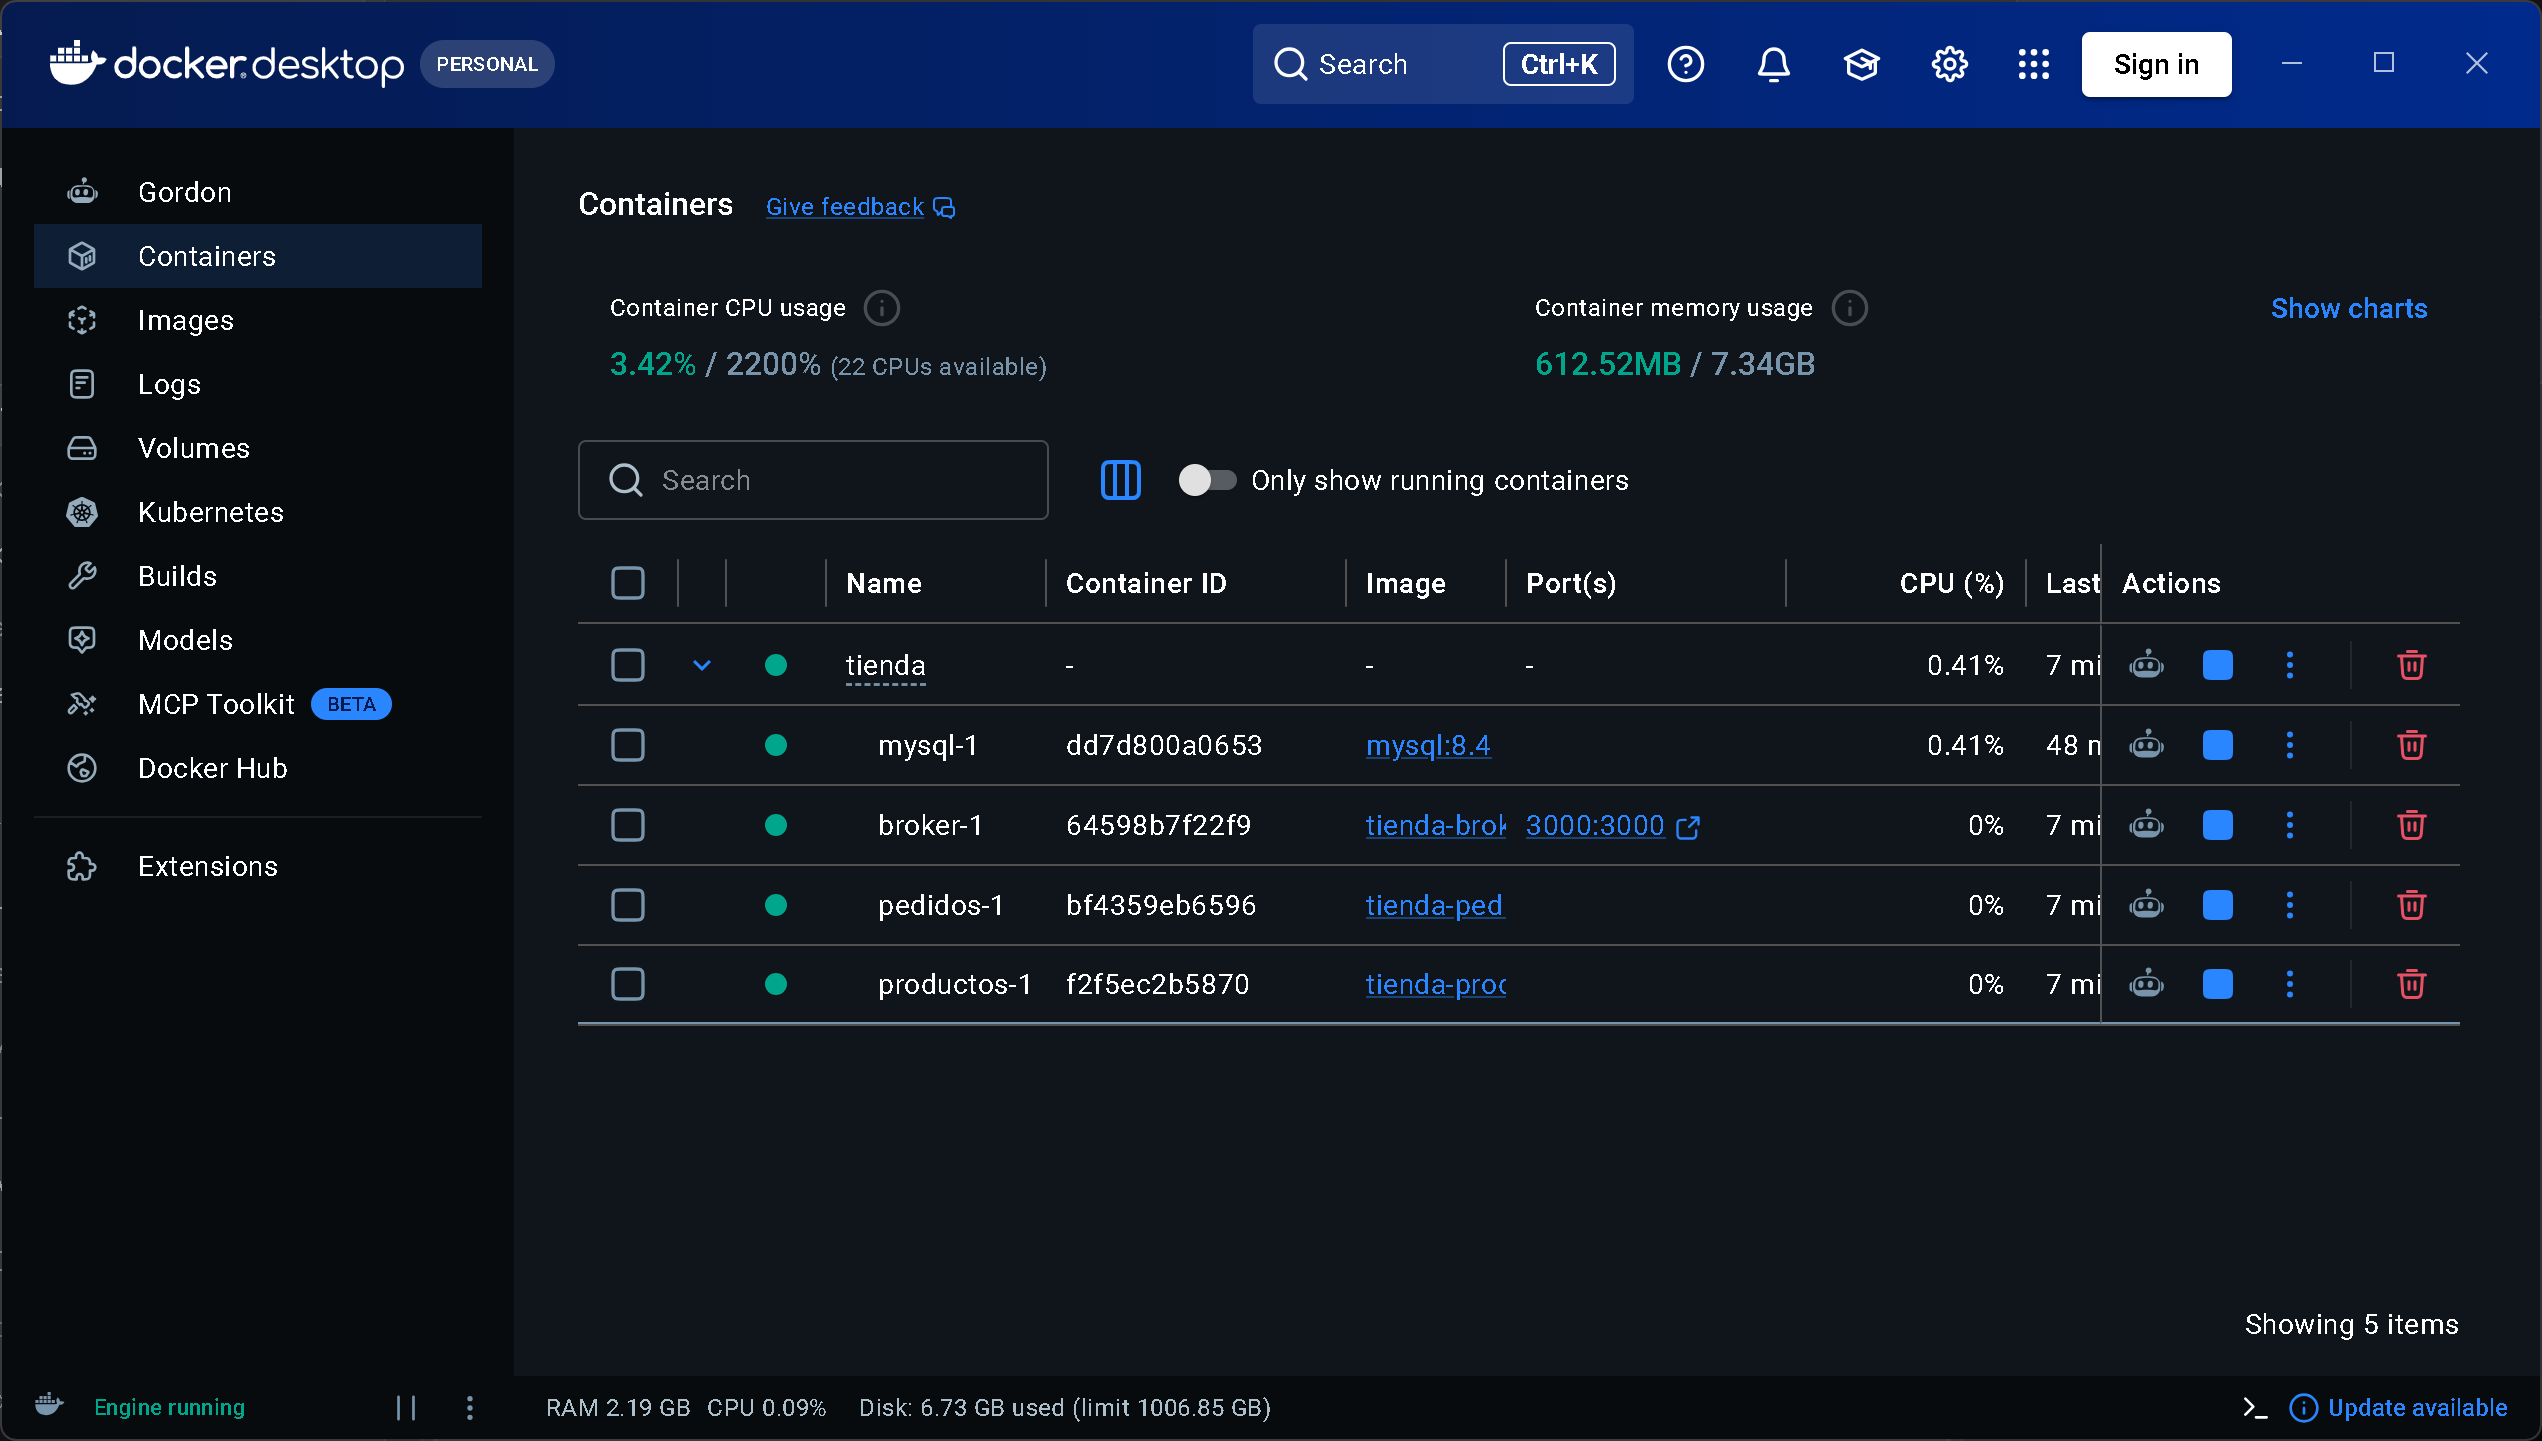
\includegraphics[width=\columnwidth]{fig/ag-docker-desktop.png}
\caption{Panel de Docker Desktop con el grupo de contenedores \texttt{tienda} expandido y en ejecución normal.}
\label{fig:docker}
\end{figure}

\section{Pruebas Funcionales y Validación en Local}

\subsection{Validación de Seguridad y Rechazo Sin Token}
Para verificar el cumplimiento del criterio de seguridad del mediador, se realizaron pruebas contra la ruta protegida \texttt{http://localhost:3000/productos} prescindiendo de cabeceras de autorización.

Como se documenta en la Fig.~\ref{fig:postman}, el Broker interceptó inmediatamente la petición y emitió una respuesta con código de estado HTTP \textbf{401 Unauthorized}, retornando el cuerpo JSON estructurado:
\begin{lstlisting}[language=json]
{
  "message": "Token ausente, inválido o expirado",
  "error": "Unauthorized",
  "statusCode": 401
}
\end{lstlisting}
Esto corrobora empíricamente que ninguna solicitud sin credenciales válidas logra penetrar hacia el microservicio interno de productos.

\begin{figure}[htbp]
\centering
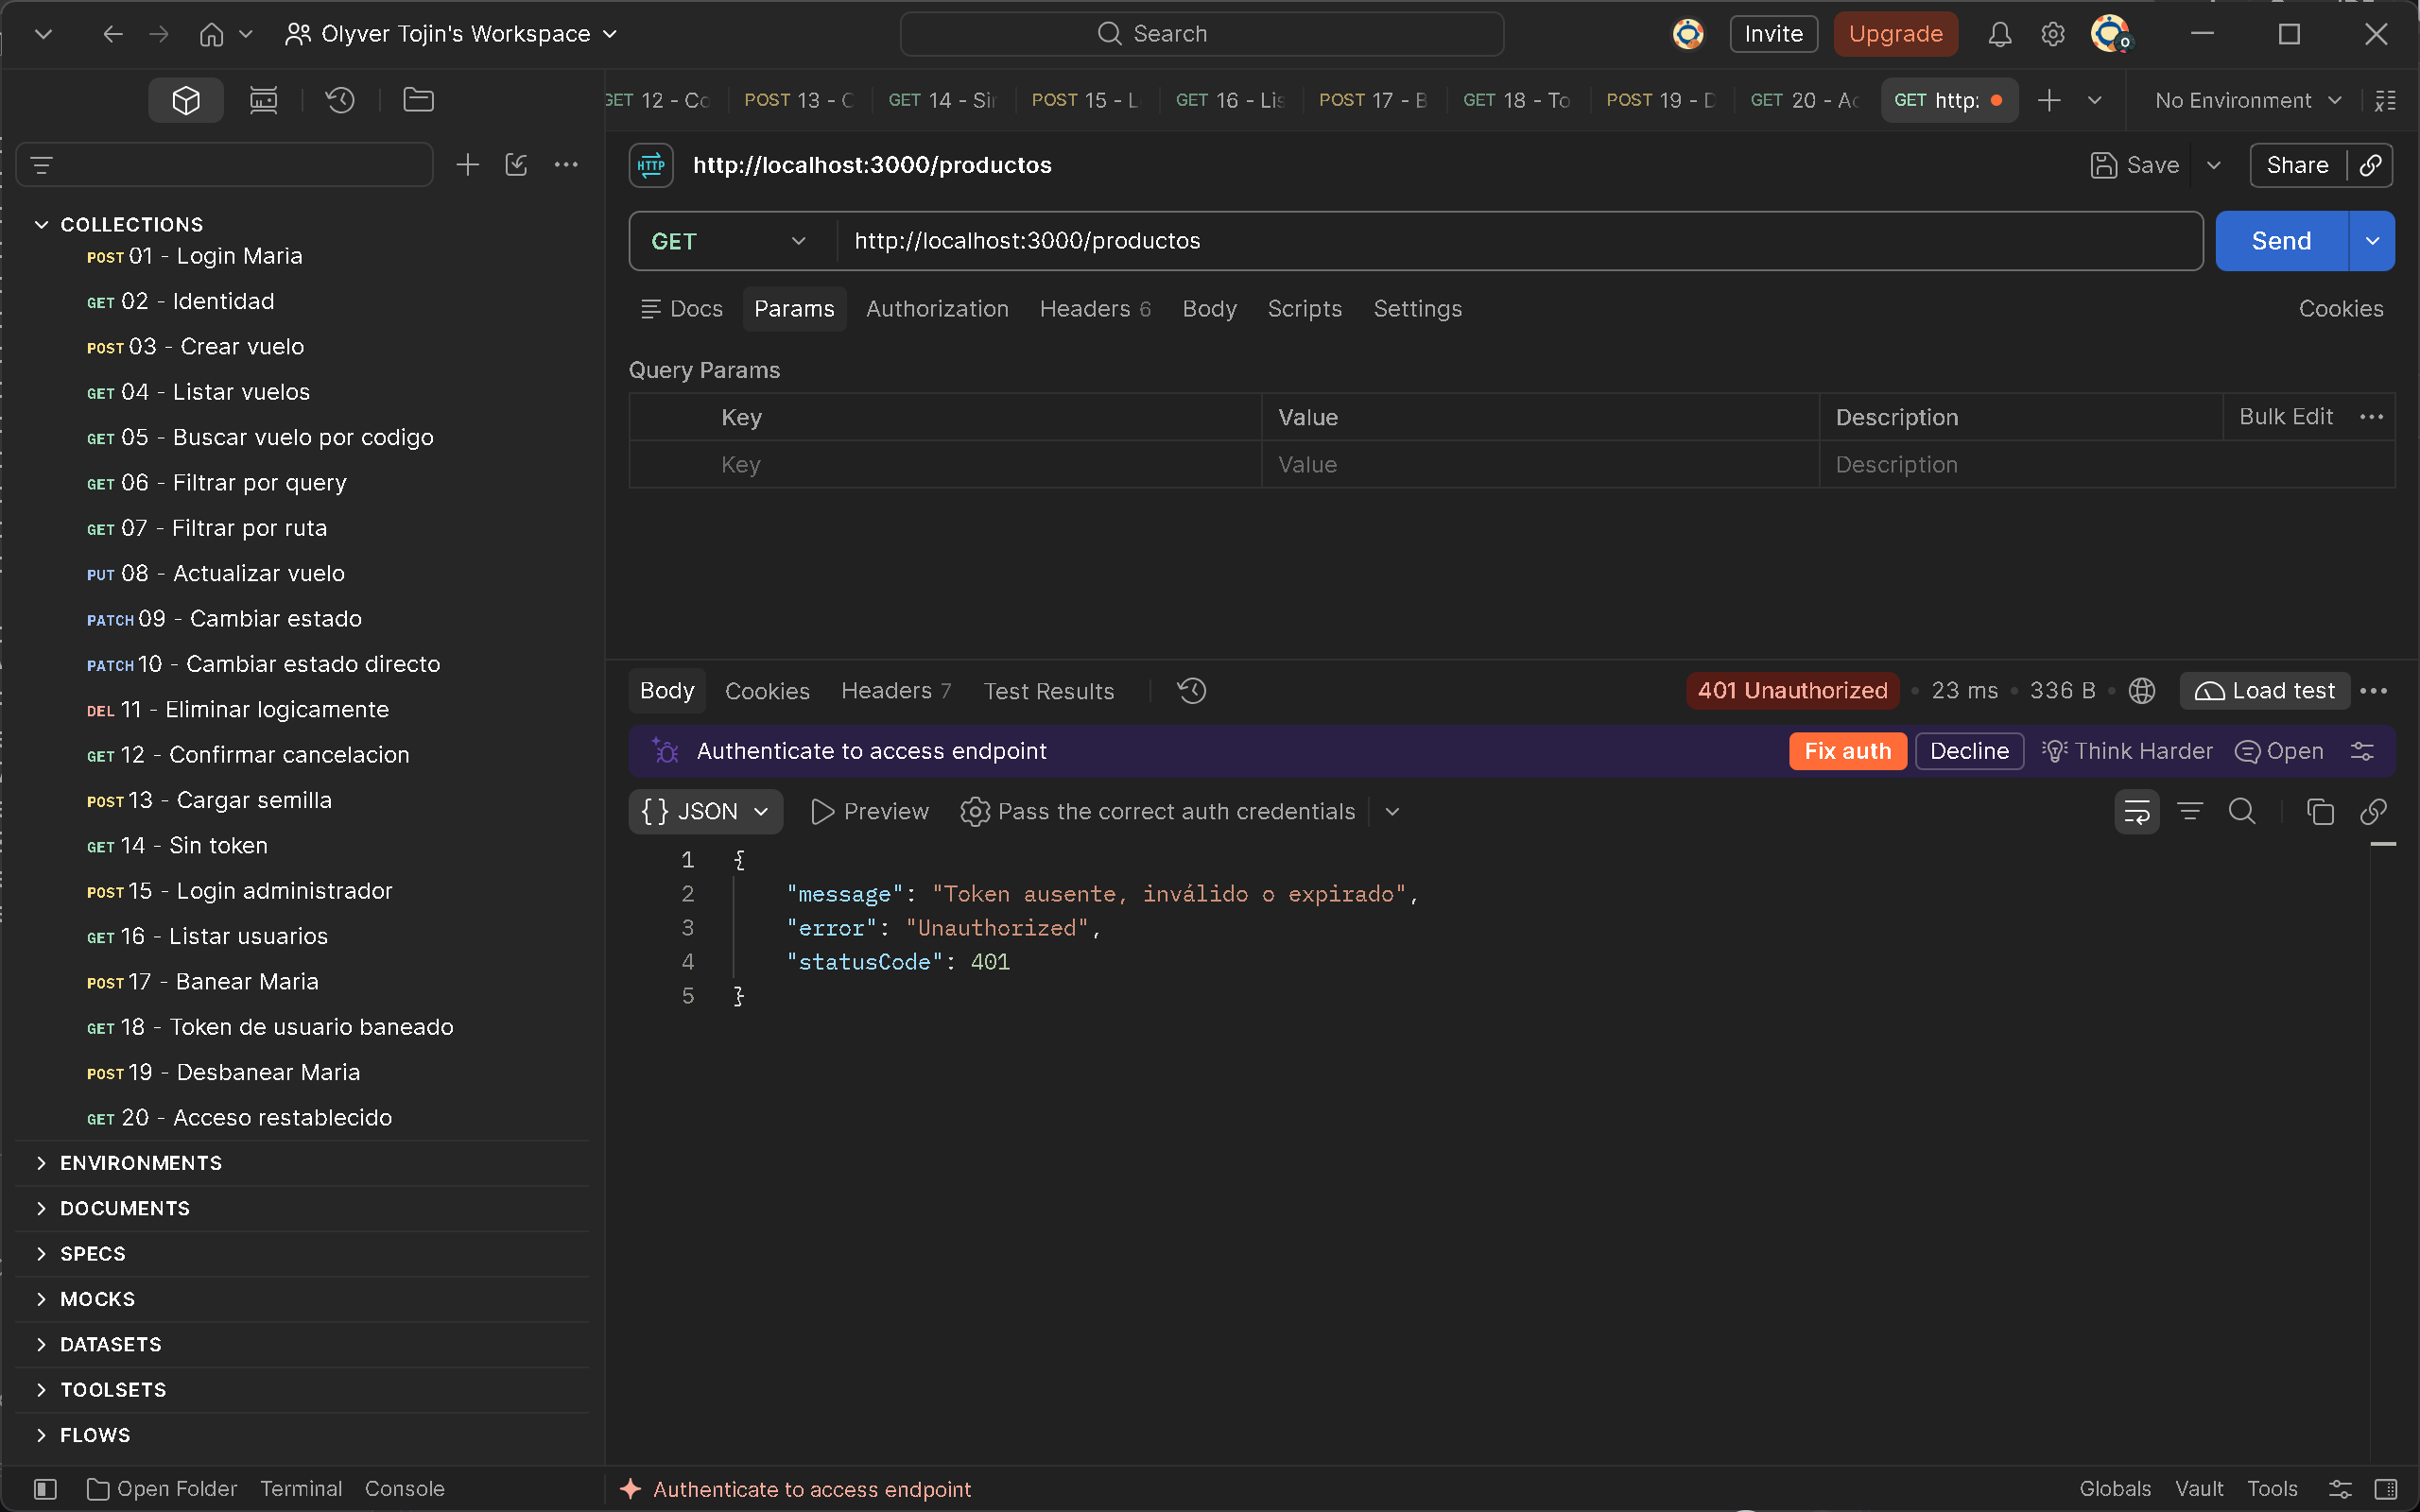
\includegraphics[width=\columnwidth]{fig/ag-postman.png}
\caption{Prueba en Postman dirigida a \texttt{http://localhost:3000/productos} sin token de autorización, demostrando el rechazo 401 Unauthorized.}
\label{fig:postman}
\end{figure}

\subsection{Pruebas Unitarias Mediante Mocks}
En cumplimiento con los requerimientos funcionales de la cátedra, se implementaron suites de pruebas unitarias automatizadas basadas en dobles de prueba (\textit{mocks}) utilizando el módulo nativo \texttt{node:test} y las utilidades \texttt{t.mock.fn} de Node.js:
\begin{itemize}
    \item \textbf{Confirmación de Pedido:} Se simuló la respuesta afirmativa del microservicio de productos ($stock=5$), verificando que la orden transiciona a estado \texttt{CONFIRMADO} y descuenta la cantidad exacta.
    \item \textbf{Rechazo por Stock Insuficiente:} Se mockeó una disponibilidad menor a la demanda, comprobando que la capa de dominio dispara una excepción \texttt{ConflictException} y cancela la llamada a descuento.
    \item \textbf{Tolerancia a Timeout:} Se simuló una caída o demora del microservicio de catálogo lanzando \texttt{GatewayTimeoutException}, validando que el pedido permanece en estado \texttt{PENDIENTE} para garantizar idempotencia en reintentos.
\end{itemize}

\subsection{Matriz de Endpoints y Cobertura Postman}
Se estructuró una colección de Postman con 20 escenarios de prueba automatizados mediante Newman, evaluando:
\begin{enumerate}
    \item Generación de JWT tras autenticación en \texttt{POST /auth/login}.
    \item Inserción y lectura de catálogo mediante \texttt{POST /productos} y \texttt{GET /productos}.
    \item Flujo transaccional de compra en \texttt{POST /pedidos}.
    \item Validación de existencias posteriores al descuento.
    \item Manejo de casos de borde: precios negativos ($400$), producto inexistente ($404$) y stock agotado ($409$).
\end{enumerate}

\section{Estado de Avance Frente a la Rúbrica}
La Tabla~\ref{tab:rubrica} resume la correspondencia entre los criterios de evaluación estipulados en el enunciado del proyecto final y los componentes consolidados en este informe de avance.

\begin{table}[htbp]
\caption{Matriz de Cumplimiento de la Rúbrica de Evaluación}
\begin{center}
\begin{tabular}{p{3.2cm}cp{3.8cm}}
\toprule
\textbf{Criterio Evaluado} & \textbf{Puntos} & \textbf{Estado en el Presente Avance} \\
\midrule
Arquitectura general (3 servicios independientes con su propia arquitectura) & 4 pts & Completado: Broker (Mediator), Productos (MVC) y Pedidos (Capas). \\
\midrule
Autenticación por token en Broker (Rechazo sin token válido) & 2 pts & Completado: Verificado en Postman con HTTP 401 y JWT de sesión. \\
\midrule
Comunicación correcta entre servicios & 3 pts & Completado: Pedidos invoca a Productos pasando obligatoriamente por Broker. \\
\midrule
Pruebas unitarias con mocks & 2 pts & Completado: Cobertura de casos exitosos, conflicto de stock y timeout. \\
\midrule
Documentación vía Swagger & 1 pt & Implementado: Módulos \texttt{@nestjs/swagger} configurados por servicio. \\
\midrule
Publicación en la nube (VPS) & 2 pts & Fase siguiente: En preparación para el despliegue final. \\
\midrule
Demostración individual & 1 pt & Fase final: Preparada con colección de Postman. \\
\bottomrule
\end{tabular}
\label{tab:rubrica}
\end{center}
\end{table}

\section{Conclusiones y Próximos Pasos}
La puesta en marcha local ha validado satisfactoriamente los pilares de desacoplamiento, seguridad y contención de datos requeridos para el proyecto final de Arquitectura de Sistemas I. El uso de Docker Compose ha simplificado el ciclo de vida de los servicios y ha garantizado que el microservicio Broker cumpla rigurosamente su función como compuerta única de entrada.

Los próximos pasos contemplan:
\begin{enumerate}
    \item Aprovisionamiento y despliegue del ecosistema en el servidor virtual en la nube (VPS).
    \item Configuración de nombres de dominio y certificados SSL/TLS para el acceso seguro al broker público.
    \item Ejecución de la suite completa de pruebas Newman para la entrega y demostración individual ante el docente.
\end{enumerate}

\begin{thebibliography}{00}
\bibitem{fowler} M. Fowler, ``Microservices: a definition of this new architectural term,'' \textit{martinfowler.com}, 2014.
\bibitem{newman} S. Newman, \textit{Building Microservices: Designing Fine-Grained Systems}, 2nd ed. Sebastopol, CA: O'Reilly Media, 2021.
\bibitem{gamma} E. Gamma, R. Helm, R. Johnson, and J. Vlissides, \textit{Design Patterns: Elements of Reusable Object-Oriented Software}. Reading, MA: Addison-Wesley, 1994.
\bibitem{ieee42010} IEEE, ``ISO/IEC/IEEE Systems and software engineering -- Architecture description,'' \textit{ISO/IEC/IEEE 42010:2011}, 2011.
\end{thebibliography}

\end{document}
